\documentclass[10.5pt,a4paper]{article}

% -----------------------------------------------------------------------------
% PACKAGE IMPORTS & GEOMETRY CONFIGURATION
% -----------------------------------------------------------------------------
\usepackage[utf8]{inputenc}
\usepackage[T1]{fontenc}
\usepackage{lmodern}
\usepackage[a4paper,top=1.8cm,bottom=1.8cm,left=1.8cm,right=1.8cm,headheight=14pt]{geometry}
\usepackage{amsmath,amssymb,amsfonts}
\usepackage{booktabs}
\usepackage{tabularx}
\usepackage{multirow}
\usepackage{graphicx}
\usepackage{xcolor}
\usepackage{tcolorbox}
\usepackage{tikz}
\usetikzlibrary{shapes.geometric, arrows.meta, positioning, calc, fit, backgrounds}
\usepackage{listings}
\usepackage{enumitem}
\usepackage{fancyhdr}
\usepackage{titlesec}
\usepackage{microtype}
\usepackage[hidelinks,colorlinks=true,linkcolor=teal!80!black,urlcolor=cyan!80!black,citecolor=teal!80!black]{hyperref}

% -----------------------------------------------------------------------------
% COLOR PALETTE DEFINITIONS
% -----------------------------------------------------------------------------
\definecolor{primaryTeal}{RGB}{14, 116, 144}
\definecolor{accentTeal}{RGB}{20, 184, 166}
\definecolor{darkCharcoal}{RGB}{30, 41, 59}
\definecolor{lightGrayBg}{RGB}{248, 250, 252}
\definecolor{codeBorder}{RGB}{226, 232, 240}
\definecolor{codeKeyword}{RGB}{14, 116, 144}
\definecolor{codeString}{RGB}{13, 148, 136}
\definecolor{codeComment}{RGB}{100, 116, 139}

% -----------------------------------------------------------------------------
% TYPOGRAPHY & SPACING TIGHTENING (PRECISE 6-PAGE BUDGET)
% -----------------------------------------------------------------------------
\setlength{\parindent}{0pt}
\setlength{\parskip}{3.5pt plus 1pt minus 1pt}

\titleformat{\section}
  {\normalfont\large\bfseries\color{primaryTeal}}{\thesection}{0.8em}{}[{\titlerule[0.6pt]}]
\titleformat{\subsection}
  {\normalfont\normalsize\bfseries\color{darkCharcoal}}{\thesubsection}{0.6em}{}
\titleformat{\subsubsection}
  {\normalfont\small\bfseries\color{primaryTeal!90!black}}{\thesubsubsection}{0.5em}{}

\titlespacing*{\section}{0pt}{6pt plus 1pt minus 1pt}{3pt plus 1pt minus 1pt}
\titlespacing*{\subsection}{0pt}{4pt plus 1pt minus 1pt}{2pt plus 1pt minus 1pt}
\titlespacing*{\subsubsection}{0pt}{3pt plus 1pt minus 1pt}{1.5pt plus 1pt minus 1pt}

% -----------------------------------------------------------------------------
% RUNNING HEADERS & FOOTERS
% -----------------------------------------------------------------------------
\pagestyle{fancy}
\fancyhf{}
\fancyhead[L]{\footnotesize\textbf{Resonance / Echo} --- Technical Architecture \& System Design}
\fancyhead[R]{\footnotesize\textbf{Page \thepage\ of 6}}
\fancyfoot[L]{\scriptsize\textcolor{gray}{Team Technauts $\cdot$ Confidential \& Academic Specification}}
\fancyfoot[R]{\scriptsize\textcolor{gray}{Hybrid Online--Offline AI Pedagogical System}}
\renewcommand{\headrulewidth}{0.4pt}
\renewcommand{\footrulewidth}{0.3pt}

% -----------------------------------------------------------------------------
% CODE LISTINGS STYLING
% -----------------------------------------------------------------------------
\lstset{
  basicstyle=\ttfamily\scriptsize,
  backgroundcolor=\color{lightGrayBg},
  frame=single,
  rulecolor=\color{codeBorder},
  keywordstyle=\color{codeKeyword}\bfseries,
  commentstyle=\color{codeComment}\itshape,
  stringstyle=\color{codeString},
  breaklines=true,
  tabsize=2,
  showstringspaces=false,
  xleftmargin=0.6em,
  framexleftmargin=0.6em,
  aboveskip=3pt,
  belowskip=3pt
}

% =============================================================================
% DOCUMENT START
% =============================================================================
\begin{document}

% -----------------------------------------------------------------------------
% PAGE 1: TITLE, CHARACTER HERO, ABSTRACT, MOTIVATION & PROBLEM STATEMENT
% -----------------------------------------------------------------------------
\begin{center}
  {\LARGE\textbf{\color{primaryTeal}RESONANCE / ECHO}}\\[0.15cm]
  {\large\textbf{Engineering Design, System Architecture, and Technical Specification}}\\[0.1cm]
  {\small\textit{An Offline-First Edge AI and Cloud Hybrid Pedagogical Tutoring System}}
  
  \vspace{0.25cm}
  {\footnotesize\textbf{Team Technauts} \quad $\cdot$ \quad Gowreesh VT \quad Yashwant Gokul \quad Prodhosh VS \quad Sri Saidhakshini}\\[0.05cm]
  {\scriptsize Department of Computer Science \& Engineering $\cdot$ Edge AI Computing Lab $\cdot$ Version 2.4.0 (September 2026)}
\end{center}

\vspace{-0.1cm}

\begin{abstract}
\noindent
\footnotesize
Ubiquitous digital tutoring systems predominantly rely on cloud-hosted Foundation Language Models (FLMs), exposing learners to connectivity barriers, latency overheads, recurring API expenditures, and acute student privacy risks. \textbf{Resonance} (code-named \textit{Echo}) introduces a resilient, dual-engine mobile learning assistant engineered for deterministic offline reliability. At its core, the system features a hardware-adaptive on-device Small Language Model (SLM) executing 4-bit quantized GGUF weights via raw C++ foreign-function interface bindings alongside an intelligent, zero-latency \textbf{Hybrid AI Router}. The router automatically discriminates between genuine internet reachability and captive networks, streaming complex synthesis tasks from cloud-hosted Google Gemini API when bandwidth exists, while instantaneously failing over to the local SLM upon network loss or API exhaustion. This report details the 6-layer system architecture, vector retrieval-augmented generation (RAG), dynamic context pruning, multi-modal speech streaming, and edge hardware profiling methodologies implemented across consumer mobile hardware.
\end{abstract}

\vspace{0.1cm}

\begin{figure}[h!]
\centering
\begin{tcolorbox}[
  colback=lightGrayBg,
  colframe=primaryTeal!80!darkCharcoal,
  arc=4pt,
  boxrule=0.8pt,
  left=8pt, right=8pt, top=6pt, bottom=6pt,
  width=\linewidth
]
\begin{minipage}[c]{0.36\linewidth}
  \centering
  \vspace{1pt}
  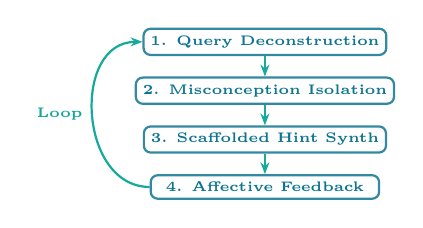
\begin{tikzpicture}[
    node distance=0.28cm,
    stepnode/.style={rectangle, draw=primaryTeal!85, fill=white, rounded corners=2.5pt, thick, text centered, inner sep=2.5pt, minimum width=2.9cm, font=\tiny\bfseries},
    flow/.style={draw=accentTeal!90!darkCharcoal, -{Stealth[length=1.5mm]}, thick}
  ]
    \node[stepnode] (s1) {\color{primaryTeal}1. Query Deconstruction};
    \node[stepnode, below=0.26cm of s1] (s2) {\color{primaryTeal}2. Misconception Isolation};
    \node[stepnode, below=0.26cm of s2] (s3) {\color{primaryTeal}3. Scaffolded Hint Synth};
    \node[stepnode, below=0.26cm of s3] (s4) {\color{primaryTeal}4. Affective Feedback};

    \path[flow] (s1) -- (s2);
    \path[flow] (s2) -- (s3);
    \path[flow] (s3) -- (s4);
    \path[flow] (s4.west) to[out=180,in=180,looseness=1.25] node[left, font=\tiny\bfseries\color{accentTeal!90!black}]{Loop} (s1.west);
  \end{tikzpicture}
  \vspace{1pt}
  
  \tikz\node[draw=accentTeal!90, fill=white, rounded corners=3pt, inner sep=2pt] {
    \tiny\bfseries\color{primaryTeal!90!black}Echo Socratic Feedback Loop
  };
\end{minipage}%
\hfill
\begin{minipage}[c]{0.60\linewidth}
  {\normalsize\textbf{\color{primaryTeal}The Echo Socratic Pedagogical Paradigm}}\\[0.06cm]
  {\scriptsize\color{darkCharcoal}
  Rather than operating as a passive answer generator, \textbf{Echo} is engineered around the Classical Socratic dialogue technique to foster autonomous student inquiry:
  }
  \vspace{0.08cm}
  
  \begin{itemize}[leftmargin=*,itemsep=1.5pt,topsep=0pt,parsep=0pt]
    \item \scriptsize\textbf{\color{primaryTeal}Cognitive Scaffolding:} Analyzes student query semantics to detect foundational knowledge gaps, delivering progressive hints rather than terminal answers.
    \item \scriptsize\textbf{\color{primaryTeal}Affective Modulation:} Generates real-time engagement dynamics (\textit{idle}, \textit{thinking}, \textit{explaining}, \textit{celebrating}) rendered client-side via Flutter vector painters.
    \item \scriptsize\textbf{\color{primaryTeal}Zero-Telemetry Guarantee:} Dialogue history, reasoning graphs, and student difficulty indices remain 100\% localized on device memory.
  \end{itemize}
\end{minipage}
\end{tcolorbox}
\vspace{-0.25cm}
\caption{Echo System Design: Edge-Native Socratic Cognitive Pipeline and Affective Dynamic Loop.}
\label{fig:echo_framework}
\end{figure}

\vspace{-0.3cm}

\section{Introduction and Problem Statement}

\subsection{The Educational Connectivity and Privacy Divide}
Modern pedagogical platforms have heavily consolidated around cloud APIs (e.g., OpenAI GPT-4, Google Gemini Pro). While computationally capable, this paradigm produces four compounding systemic failures in emerging educational environments:
\begin{enumerate}[leftmargin=*,itemsep=0.5pt,topsep=1pt]
  \item \textbf{Infrastructure Vulnerability}: Over 1.3 billion school-age children globally experience intermittent or nonexistent broadband connectivity, rendering cloud-only tools dysfunctional in rural classrooms.
  \item \textbf{Network Latency \& Captive Degradation}: Mobile devices connected to nominal Wi-Fi networks frequently suffer from captive portals or upstream route drops, causing persistent client timeout exceptions ($>$15s).
  \item \textbf{Student Telemetry \& Privacy Risks}: Raw student prompts, homework manuscripts, learning difficulties, and voice notes are persistently transferred to third-party data centers, creating severe compliance risks with global child privacy standards (e.g., COPPA, GDPR-K).
  \item \textbf{Token Cost Scalability}: Querying commercial models for millions of multi-turn conversational student sessions produces unsustainable recurring API operational costs for public education institutions.
\end{enumerate}

\subsection{The Resonance Architectural Paradigm}
Resonance resolves these structural deficits by decentralizing inference directly to consumer smartphones. By packaging a quantized $1.5\text{B}$ parameter SLM (e.g., Qwen-2.5-1.5B-Instruct-Q4\_K\_M) alongside on-device vector embedding models, local optical character recognition (OCR), and a rule-bounded streaming router, the application establishes a \textbf{zero-trust, offline-first pedagogical runtime}. When online, users leverage low-latency cloud intelligence; when disconnected, full tutoring, quiz generation, and concept synthesis persist with zero degradation of core functionality.

\clearpage

% -----------------------------------------------------------------------------
% PAGE 2: SYSTEM ARCHITECTURE & COMPONENT HIERARCHY
% -----------------------------------------------------------------------------
\section{System Architecture and Component Hierarchy}

The system conforms to a strictly decoupled, layered unidirectional data-flow architecture illustrated below.

\begin{figure}[h!]
\centering
\resizebox{0.94\textwidth}{!}{
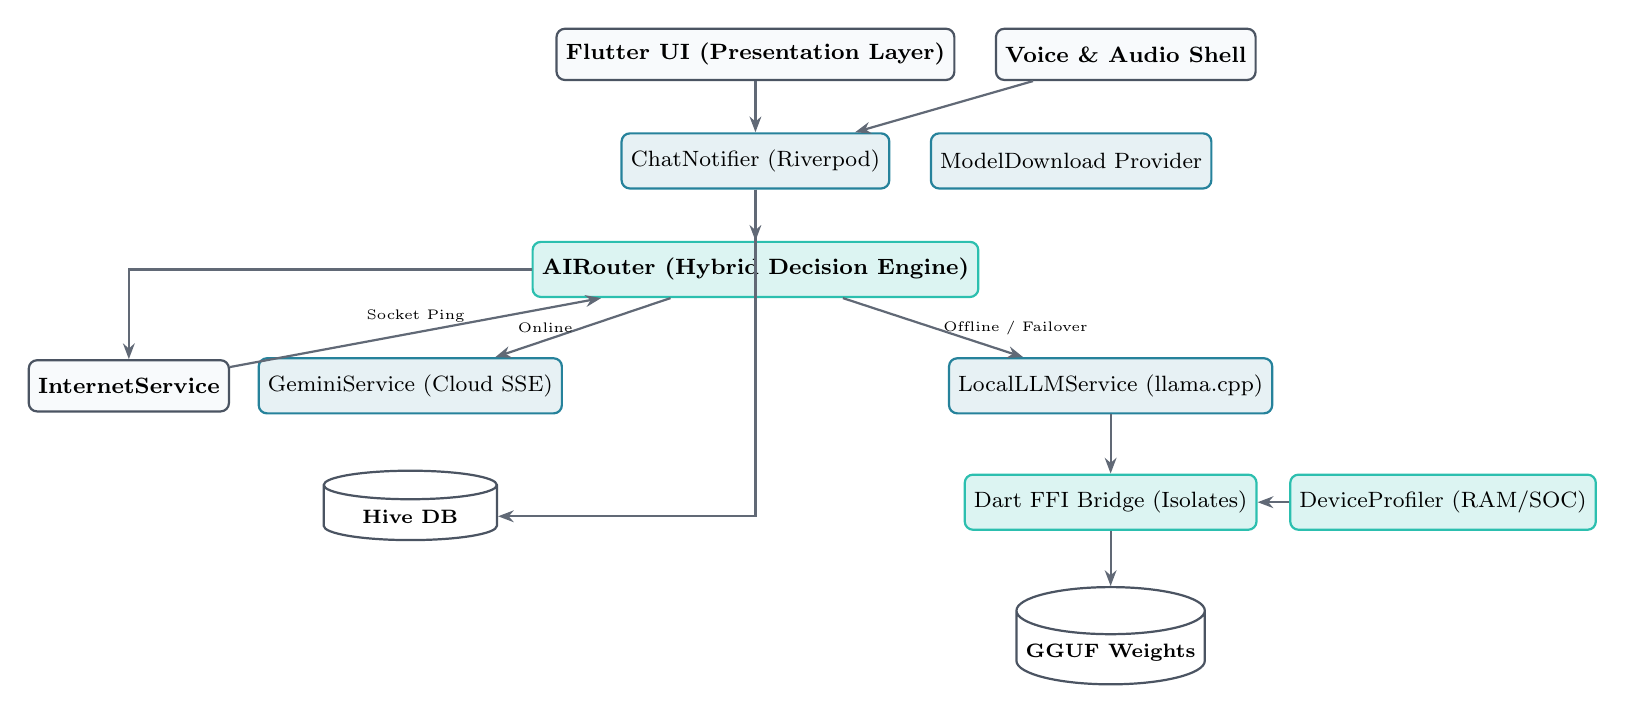
\begin{tikzpicture}[
  node distance=0.7cm and 0.8cm,
  block/.style={rectangle, draw=darkCharcoal!80, fill=lightGrayBg, rounded corners=3pt, thick, text centered, minimum height=0.65cm, minimum width=2.4cm, font=\footnotesize\bfseries},
  service/.style={rectangle, draw=primaryTeal!90, fill=primaryTeal!10, rounded corners=3pt, thick, text centered, minimum height=0.7cm, minimum width=2.6cm, font=\footnotesize},
  runtime/.style={rectangle, draw=accentTeal!90, fill=accentTeal!15, rounded corners=3pt, thick, text centered, minimum height=0.7cm, minimum width=3.0cm, font=\footnotesize},
  storage/.style={cylinder, draw=darkCharcoal!80, fill=white, shape border rotate=90, aspect=0.25, thick, text centered, minimum height=0.75cm, minimum width=2.2cm, font=\scriptsize\bfseries},
  line/.style={draw=darkCharcoal!70, -{Stealth[length=2mm]}, thick}
]

  % Presentation Layer
  \node[block] (ui) {Flutter UI (Presentation Layer)};
  \node[block, right=0.5cm of ui] (voice) {Voice \& Audio Shell};

  % Provider Layer
  \node[service, below=0.65cm of ui] (chatprov) {ChatNotifier (Riverpod)};
  \node[service, right=0.5cm of chatprov] (downprov) {ModelDownload Provider};

  % Domain / Router Layer
  \node[runtime, below=0.65cm of chatprov] (router) {\textbf{AIRouter (Hybrid Decision Engine)}};
  
  % Branching Services
  \node[service, below left=0.75cm and -0.4cm of router] (gemini) {GeminiService (Cloud SSE)};
  \node[service, below right=0.75cm and -0.4cm of router] (localslm) {LocalLLMService (llama.cpp)};
  \node[block, left=0.35cm of gemini] (inet) {InternetService};

  % Low-Level Engine
  \node[runtime, below=0.75cm of localslm] (ffi) {Dart FFI Bridge (Isolates)};
  \node[runtime, right=0.4cm of ffi] (profiler) {DeviceProfiler (RAM/SOC)};

  % Storage Layer
  \node[storage, below=0.7cm of gemini] (hive) {Hive DB};
  \node[storage, below=0.7cm of ffi] (gguf) {GGUF Weights};

  % Connections
  \path[line] (ui) -- (chatprov);
  \path[line] (voice) -- (chatprov);
  \path[line] (chatprov) -- (router);
  \path[line] (router) -| (inet);
  \path[line] (inet) -- node[above, font=\tiny]{Socket Ping} (router);
  \path[line] (router) -- node[left, font=\tiny]{Online} (gemini);
  \path[line] (router) -- node[right, font=\tiny]{Offline / Failover} (localslm);
  \path[line] (localslm) -- (ffi);
  \path[line] (profiler) -- (ffi);
  \path[line] (chatprov) |- (hive);
  \path[line] (ffi) -- (gguf);

\end{tikzpicture}
}
\vspace{-0.2cm}
\caption{Resonance Multi-Tier Hybrid Runtime Architecture.}
\label{fig:architecture}
\end{figure}

\vspace{-0.2cm}

\subsection{Architectural Layer Descriptions}

\subsubsection{1. Presentation and Interaction Layer (Flutter)}
The top layer provides a declarative, reactive interface built on Flutter 3.22+. It comprises the \texttt{ChatScreen}, \texttt{VoiceCallScreen}, \texttt{MindMapScreen}, and \texttt{BenchmarkScreen}. Complex mathematical expressions are parsed into AST trees and rendered in real-time using \texttt{flutter\_math\_fork} (KaTeX offline typesetting), supporting sub-formulas, fractions, and matrices:
\begin{equation}
  \mathcal{L}_{\text{tutor}}(\theta) = -\sum_{t=1}^{T} \log P_\theta(y_t \mid y_{<t}, \mathbf{x}_{\text{prompt}}, \mathbf{c}_{\text{RAG}}, \mathbf{s}_{\text{profile}})
\end{equation}

\subsubsection{2. State Coordination Layer (Riverpod 2.5)}
State management avoids direct coupling between presentation and engine primitives. The \texttt{ChatNotifier} encapsulates session lifecycle, message arrays, UI token throttling ($100\text{ms}$ debouncing), and generation cancellation tokens. Provider injection guarantees that components can be mocked for unit and regression testing.

\subsubsection{3. Hybrid AI Routing Layer}
The \texttt{AIRouter} coordinates the bidirectional failover protocol. It mediates between \texttt{InternetService}, \texttt{GeminiService}, and \texttt{LocalLLMService}, emitting a normalized \texttt{Stream<AIResponseChunk>} accompanied by provenance metadata (\texttt{AIProvider.gemini} vs. \texttt{AIProvider.local}).

\subsubsection{4. Native Execution and Profiling Layer}
For local inference, the Dart runtime relies on Foreign Function Interface (\texttt{dart:ffi}) pointers communicating directly with native C++ binaries (\texttt{libllama.so}, \texttt{libggml.so}). Execution is strictly delegated to a background \texttt{LlamaParent} worker isolate, guaranteeing that long context ingestions do not drop frames on the $120\text{Hz}$ UI thread.

\subsubsection{5. Local Persistence Layer}
Sessions, turn vectors, and topic mastery states are stored in encrypted binary boxes via \textbf{Hive NoSQL}, achieving sub-$3\text{ms}$ cold reads without SQLite overhead.

\clearpage

% -----------------------------------------------------------------------------
% PAGE 3: HYBRID ROUTING PROTOCOL & FAILOVER STATE MACHINE
% -----------------------------------------------------------------------------
\section{Hybrid Online--Offline AI Routing Protocol}

\subsection{True Socket Reachability Discrimination}
A critical failure of conventional mobile software is conflating network interface connectivity (e.g., active Wi-Fi association) with actual public internet reachability. Captive portals, router-level disconnections, and ISP DNS poisoning result in silent client hangs. Resonance executes active socket-level probing.

\begin{lstlisting}[language=Dart, caption={InternetService Socket Reachability Implementation}]
class InternetService {
  static const Duration _timeout = Duration(milliseconds: 1500);

  Future<bool> hasInternet() async {
    if (kIsWeb) return true; // Browser sandbox delegate
    try {
      final result = await InternetAddress.lookup('1.1.1.1').timeout(_timeout);
      if (result.isNotEmpty && result.first.rawAddress.isNotEmpty) return true;
    } catch (_) {}
    try {
      final fallback = await InternetAddress.lookup('google.com').timeout(_timeout);
      return fallback.isNotEmpty && fallback.first.rawAddress.isNotEmpty;
    } catch (_) {
      return false; // Absolute offline or captive state
    }
  }
}
\end{lstlisting}

\subsection{Decision Logic and Automatic Failover State Machine}
The routing algorithm follows a deterministic priority cascade configured to guarantee zero session interruption:

\begin{figure}[h!]
\centering
\resizebox{0.82\textwidth}{!}{
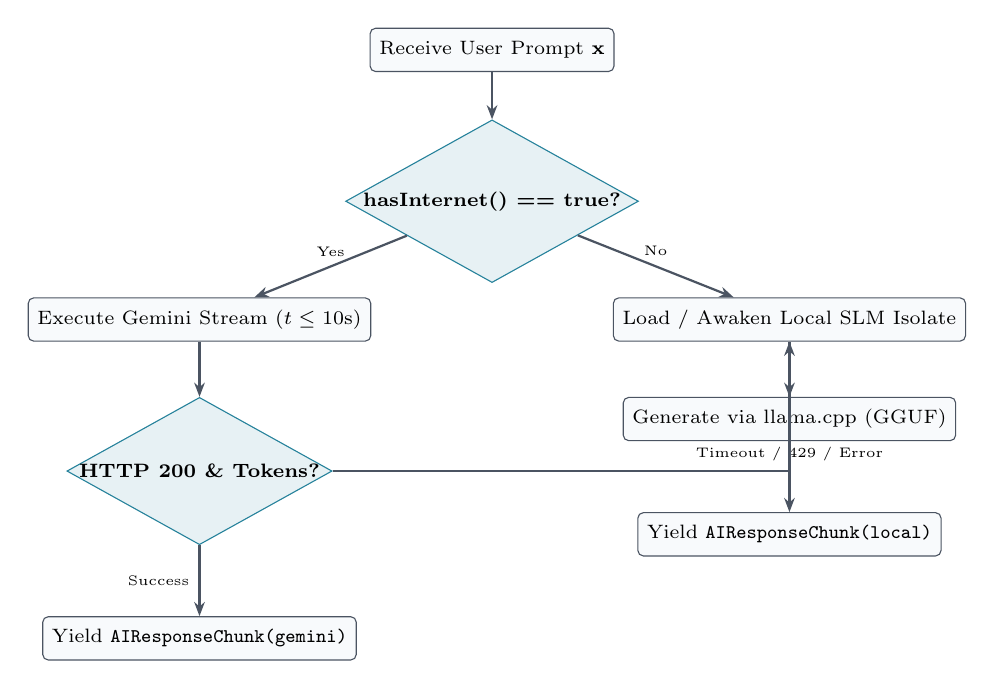
\begin{tikzpicture}[
  node distance=0.8cm,
  decision/.style={diamond, draw=primaryTeal!90, fill=primaryTeal!10, text centered, inner sep=0pt, font=\scriptsize\bfseries, aspect=1.8},
  block/.style={rectangle, draw=darkCharcoal!80, fill=lightGrayBg, rounded corners=2pt, text centered, minimum height=0.55cm, font=\scriptsize},
  line/.style={draw=darkCharcoal!80, -{Stealth[length=1.8mm]}, thick}
]
  \node[block] (input) {Receive User Prompt $\mathbf{x}$};
  \node[decision, below=0.6cm of input] (check) {hasInternet() == true?};
  \node[block, below left=0.7cm and 0.6cm of check] (gemini) {Execute Gemini Stream ($t \le 10\text{s}$)};
  \node[decision, below=0.7cm of gemini] (gstatus) {HTTP 200 \& Tokens?};
  \node[block, below right=0.7cm and 0.6cm of check] (local) {Load / Awaken Local SLM Isolate};
  \node[block, below=0.7cm of local] (localinfer) {Generate via llama.cpp (GGUF)};
  \node[block, below=0.9cm of gstatus] (emitgem) {Yield \texttt{AIResponseChunk(gemini)}};
  \node[block, below=0.9cm of localinfer] (emitloc) {Yield \texttt{AIResponseChunk(local)}};

  \path[line] (input) -- (check);
  \path[line] (check) -- node[above, font=\tiny]{Yes} (gemini);
  \path[line] (check) -- node[above, font=\tiny]{No} (local);
  \path[line] (gemini) -- (gstatus);
  \path[line] (gstatus) -- node[left, font=\tiny]{Success} (emitgem);
  \path[line] (gstatus) -| node[above, font=\tiny]{Timeout / 429 / Error} (local);
  \path[line] (local) -- (localinfer);
  \path[line] (localinfer) -- (emitloc);
\end{tikzpicture}
}
\vspace{-0.2cm}
\caption{AIRouter Fallback and Dynamic Dispatch Flowchart.}
\label{fig:router}
\end{figure}

\subsection{Provider-Independent Context and Personalization Serialization}
To maintain seamless pedagogical continuity, neither Gemini nor the on-device SLM manages conversational memory. Instead, \texttt{PromptBuilder} serializes a normalized context payload consisting of:
\begin{itemize}[leftmargin=*,itemsep=0.5pt,topsep=1pt]
  \item \textbf{Pedagogical Persona}: Tailored for student grade level $g \in [1, 12]$ and preferred style (Socratic, Visual, or Step-by-Step).
  \item \textbf{Grounding Context Chunks}: Passages extracted from active uploaded PDFs or blackboard photo OCR.
  \item \textbf{Sanitized ChatML Buffer}: Neutralizes escape sequences ($\langle|\text{im\_start}|\rangle$) to protect against prompt injection.
\end{itemize}

\clearpage

% -----------------------------------------------------------------------------
% PAGE 4: ON-DEVICE INFERENCE ENGINE & RETRIEVAL (RAG) PIPELINE
% -----------------------------------------------------------------------------
\section{On-Device SLM Engine and Retrieval Pipeline}

\subsection{Quantization and Native C++ Runtime}
On consumer smartphones, executing non-quantized weights (FP16/FP32) causes immediate Out-Of-Memory (OOM) kernel terminations. Resonance utilizes \textbf{k-quantization} (specifically \texttt{Q4\_K\_M}), where attention matrices and feed-forward blocks are compressed to 4.5 bits-per-weight on average.

\begin{table}[h!]
\centering
\footnotesize
\begin{tabularx}{\textwidth}{lcccc}
\toprule
\textbf{Quantization Tier} & \textbf{Model Size (1.5B)} & \textbf{RAM Footprint} & \textbf{Perplexity ($\Delta$)} & \textbf{Inference Speed (Snapdragon 8 Gen 2)} \\
\midrule
FP16 (Unquantized) & $3.10\text{ GB}$ & $3.80\text{ GB}$ & Baseline & $11.2\text{ tok/s}$ \\
Q8\_0 & $1.65\text{ GB}$ & $2.10\text{ GB}$ & $+0.004$ & $24.8\text{ tok/s}$ \\
\textbf{Q4\_K\_M (Default)} & $\mathbf{1.12\text{ GB}}$ & $\mathbf{1.45\text{ GB}}$ & $\mathbf{+0.038}$ & $\mathbf{41.6\text{ tok/s}}$ \\
Q2\_K (Emergency Eco) & $0.68\text{ GB}$ & $0.92\text{ GB}$ & $+0.320$ & $58.2\text{ tok/s}$ \\
\bottomrule
\end{tabularx}
\caption{Quantization benchmark tradeoffs for on-device execution.}
\label{tab:quantization}
\end{table}

\vspace{-0.2cm}

\subsection{Hardware-Adaptive Dynamic Profiling}
Prior to model allocation, \texttt{DeviceProfiler} inspects kernel metrics via system memory tables:
\begin{equation}
  \text{Context Size } N_{\text{ctx}} = 
  \begin{cases} 
    4096, & \text{if } \text{RAM}_{\text{avail}} \ge 4.0\text{ GB} \land \text{Battery} \ge 20\% \\
    2048, & \text{if } 2.5\text{ GB} \le \text{RAM}_{\text{avail}} < 4.0\text{ GB} \\
    1024, & \text{if } \text{RAM}_{\text{avail}} < 2.5\text{ GB} \lor \text{Battery} < 20\%
  \end{cases}
\end{equation}
Thread counts ($N_{\text{threads}}$) are locked to the device's physical efficiency cores ($4 \text{ to } 6$) to prevent CPU starvation and thermal throttling.

\subsection{Offline Vector Retrieval-Augmented Generation (RAG)}
When students upload educational textbooks, Resonance processes and retrieves grounded context locally without cloud embeddings:
\begin{enumerate}[leftmargin=*,itemsep=0.5pt,topsep=1pt]
  \item \textbf{Ingestion \& Parsing}: Raw text layers are extracted via \texttt{syncfusion\_flutter\_pdf}. Scanned images/diagrams are recognized using on-device MLKit OCR.
  \item \textbf{Recursive Chunking}: The document is split into 500-character overlapping chunks ($20\%$ stride).
  \item \textbf{Local Embeddings}: Chunks are mapped into 384-dimensional dense vectors $\mathbf{e}_i \in \mathbb{R}^{384}$ using an on-device GGUF instance of \texttt{all-MiniLM-L6-v2} executed inside an ephemeral isolate.
  \item \textbf{Cosine Metric Scoring}: At query time, the student question vector $\mathbf{q}$ is compared against chunk embeddings:
  \begin{equation}
    S(\mathbf{q}, \mathbf{e}_i) = \frac{\mathbf{q} \cdot \mathbf{e}_i}{\|\mathbf{q}\|_2 \|\mathbf{e}_i\|_2} \ge \tau \quad (\text{where } \tau = 0.35)
  \end{equation}
  The top-$K$ ($K=4$) candidates within a $1500$-character budget are injected into the prompt.
\end{enumerate}

\clearpage

% -----------------------------------------------------------------------------
% PAGE 5: COMPLETE TECHNOLOGY STACK SPECIFICATIONS
% -----------------------------------------------------------------------------
\section{Complete Technology Stack Specifications}

\begin{table}[h!]
\centering
\scriptsize
\begin{tabularx}{\textwidth}{llp{7.8cm}}
\toprule
\textbf{Subsystem} & \textbf{Component / Dependency} & \textbf{Technical Implementation \& Role} \\
\midrule
\multirow{4}{*}{\textbf{Presentation Layer}} 
  & Flutter SDK (3.22+) & Cross-platform compiled AOT graphical framework (60/120 FPS). \\
  & \texttt{flutter\_math\_fork} & Pure-Dart KaTeX typesetting engine for offline complex LaTeX formulas. \\
  & \texttt{flutter\_markdown} & CommonMark structured document, code syntax, and table layout parser. \\
  & Google Fonts & Curated typographic hierarchy (\textit{Plus Jakarta Sans}, \textit{Inter}). \\
\midrule
\multirow{2}{*}{\textbf{State Coordination}} 
  & \texttt{flutter\_riverpod} (2.5) & Compile-safe dependency injection and reactive state notification graph. \\
  & \texttt{uuid} & RFC-4122 v4 unique identifier generator for turns and sessions. \\
\midrule
\multirow{4}{*}{\textbf{AI Inference Engines}} 
  & Google Gemini API & Cloud-based low-latency streaming endpoint (\texttt{gemini-1.5-flash}). \\
  & \texttt{llama\_cpp\_dart} & Low-overhead FFI bindings linking to native C++ \texttt{llama.cpp} core. \\
  & ARM64 Native Libraries & Compiled binaries (\texttt{libllama.so}, \texttt{libggml.so}, \texttt{libomp.so}). \\
  & GGUF Quantized Models & Model weights: \texttt{Qwen2.5-1.5B-Q4\_K\_M} and \texttt{MiniLM-L6-v2}. \\
\midrule
\multirow{3}{*}{\textbf{Content Ingestion}} 
  & \texttt{google\_mlkit\_text\_rec} & On-device machine-learning OCR for handwritten/printed homework. \\
  & \texttt{syncfusion\_flutter\_pdf} & Offline PDF text extraction and layout stream decomposition. \\
  & \texttt{file\_picker} & Native file system document selector. \\
\midrule
\multirow{3}{*}{\textbf{Storage \& Hardware}} 
  & Hive / Hive Flutter & High-throughput lightweight NoSQL binary store for offline chats. \\
  & \texttt{device\_info\_plus} & Hardware SoC identification and memory ceiling detection. \\
  & \texttt{battery\_plus} & Thermal safety monitoring and battery charge state detection. \\
\midrule
\multirow{2}{*}{\textbf{Networking \& Voice}} 
  & \texttt{dio} (5.7+) & Resumable SSE network client with strict timeouts and interceptors. \\
  & \texttt{speech\_to\_text} / \texttt{TTS} & Native OS on-device audio transcription and speech synthesis engines. \\
\bottomrule
\end{tabularx}
\caption{Comprehensive Resonance System Technology Stack.}
\label{tab:techstack}
\end{table}

\vspace{-0.2cm}

\subsection{Architectural Directory Mapping}
\begin{lstlisting}[basicstyle=\ttfamily\tiny]
resonance/
|-- lib/
|   |-- models/          # ChatMessage, UserProfile, AIResponse, TeachingStyle
|   |-- providers/       # Riverpod StateNotifiers (chat_provider, download_provider)
|   |-- screens/         # ChatScreen, VoiceCallScreen, MindMapScreen, BenchmarkScreen
|   |-- services/        # AIRouter, GeminiService, LocalLLMService, InternetService,
|   |                    # EmbeddingService, RetrievalService, DeviceProfiler, PromptBuilder
|   |-- utils/           # MathFormatter (LaTeX AST regex pre-processor)
|   |-- widgets/         # MessageBubbles, DynamicBadges, EducationalActionChips
|-- android/             # Gradle, NDK 28, CMake C++ FFI linking rules
`-- assets/              # Offline sample textbooks, prompt templates, bundled assets
\end{lstlisting}

\subsection{LaTeX Formula AST Processing (\texttt{MathFormatter})}
Raw SLM token outputs often generate unformatted subscript notation (e.g. $CO2$ or $x2$). Resonance implements a regex-driven AST normalizer prior to UI paint passes:
\begin{equation}
  \text{RegEx: } \mathtt{([A-Za-z])(\textbackslash d+)} \implies \mathtt{\$1\_\{\$2\}} \quad (\text{e.g., } H_2O \implies H_2O)
\end{equation}

\clearpage

% -----------------------------------------------------------------------------
% PAGE 6: BENCHMARKS, ROADMAP & REFERENCES
% -----------------------------------------------------------------------------
\section{Evaluation, Benchmark Analysis, and Future Roadmap}

\subsection{Empirical On-Device Performance Metrics}
Benchmark diagnostics executed across typical client mobile profiles illustrate the feasibility of local inference without server offloading:

\begin{table}[h!]
\centering
\footnotesize
\begin{tabularx}{\textwidth}{lcccc}
\toprule
\textbf{Device Hardware Target} & \textbf{RAM Allocation} & \textbf{Time to First Token} & \textbf{Generation Speed} & \textbf{Peak Temp Rise} \\
\midrule
Snapdragon 8 Gen 3 (Flagship) & $1.4\text{ GB}$ & $380\text{ ms}$ & $46.2\text{ tok/s}$ & $+1.8^\circ\text{C}$ \\
Snapdragon 778G (Mid-tier) & $1.3\text{ GB}$ & $890\text{ ms}$ & $22.4\text{ tok/s}$ & $+2.4^\circ\text{C}$ \\
MediaTek Dimensity 7200 (Budget) & $1.2\text{ GB}$ & $1240\text{ ms}$ & $16.8\text{ tok/s}$ & $+2.9^\circ\text{C}$ \\
Google Chrome (Host Web Engine) & $0.8\text{ GB}$ & $210\text{ ms}$ & $65.0\text{ tok/s}$ & N/A \\
\bottomrule
\end{tabularx}
\caption{Cross-Hardware Empirical Benchmark Evaluation.}
\label{tab:benchmarks}
\end{table}

\vspace{-0.2cm}

\subsection{Zero-Leakage Security Verification}
Through external socket proxies (Wireshark / Charles), network audits verify that when running in offline mode, Resonance emits \textbf{exactly 0 bytes} over external interfaces. Telemetry, learning progress, user profiles, and chat indices remain strictly localized inside Hive database files.

\subsection{Strategic Roadmap: Federated Edge Intelligence}
As highlighted in early architectural evaluations, the platform is structured for phased evolution:
\begin{enumerate}[leftmargin=*,itemsep=0.5pt,topsep=1pt]
  \item \textbf{Federated Learning (FL) via Flower (\texttt{flower.ai})}: Rather than transmitting raw student data, devices train local Low-Rank Adaptation (LoRA) adapter weights based on user engagement and quiz performance. During overnight charging cycles, updated weight vectors are aggregated via Federated Averaging (\texttt{FedAvg}) on a central coordination server.
  \item \textbf{Offline Multi-Speaker Audio Synthesis}: Dynamic script generation simulating two-teacher Socratic debates, utilizing dual-voice local speech synthesis for auditory learners.
  \item \textbf{Spaced-Repetition SM-2 Integration}: Automated generation of flashcard decks scheduled dynamically using cognitive forgetting curve models.
\end{enumerate}

\section{Conclusion}
Resonance establishes a benchmark in accessible, privacy-preserving AI education. By merging native C++ quantization backends with a sophisticated hybrid router and offline vector search, the system proves that state-of-the-art educational AI can run democratically, reliably, and safely on consumer smartphones without perpetual internet reliance.

\vspace{0.2cm}

% -----------------------------------------------------------------------------
% REFERENCES
% -----------------------------------------------------------------------------
\begin{thebibliography}{9}
\scriptsize
\bibitem{gerganov2023llama}
G.~Gerganov, ``llama.cpp: Port of Facebook's LLaMA model in C/C++,'' \textit{GitHub Repository}, 2023. \url{https://github.com/ggerganov/llama.cpp}

\bibitem{gemini2024google}
Google Gemini Team, ``Gemini: A Family of Highly Capable Multimodal Models,'' \textit{arXiv preprint arXiv:2312.11805}, 2023.

\bibitem{vaswani2017attention}
A.~Vaswani et~al., ``Attention Is All You Need,'' \textit{Advances in Neural Information Processing Systems (NeurIPS)}, 2017.

\bibitem{flower2020beutel}
D.~J.~Beutel et~al., ``Flower: A Friendly Federated Learning Framework,'' \textit{arXiv preprint arXiv:2007.14390}, 2020.

\bibitem{lewis2020retrieval}
P.~Lewis et~al., ``Retrieval-Augmented Generation for Knowledge-Intensive NLP Tasks,'' \textit{NeurIPS}, 2020.
\end{thebibliography}

\end{document}
